\documentclass{book}
\usepackage[a4paper,includeheadfoot,margin=2.54cm]{geometry}
\providecommand{\tightlist}{
\setlength{\itemsep}{0pt}\setlength{\parskip}{0pt}}
\usepackage{fontspec}
\usepackage{listings}
\usepackage[stable]{footmisc}
\usepackage{fontspec}
\lstset {language=C++}
%% Set line spacing
\usepackage{setspace}
\setstretch{1.2}
%% Disable paragraph indentation
\usepackage{parskip}
%% Start sections from new page
%\let\stdsection\section
%\renewcommand\section{\newpage\stdsection}
% Colors
\usepackage{xcolor}
%% Tango color scheme
\definecolor{SkyBlue}{HTML}{3465A4}
\definecolor{DarkSkyBlue}{HTML}{204A87}
\definecolor{Plum}{HTML}{75507B}
\definecolor{Green}{HTML}{4F8124}
\definecolor{Aluminium1}{HTML}{F8F8F8}
\definecolor{Aluminium6}{HTML}{2e3436}
\definecolor{Black}{HTML}{000000}
% Listings
\usepackage{listings}
\lstdefinestyle{myStyle}{
	belowcaptionskip=1\baselineskip,
	breaklines=true,
	frame=none,
	numbers=none, 
	basicstyle=\footnotesize\ttfamily,
	keywordstyle=\bfseries\color{green!40!black},
	commentstyle=\itshape\color{purple!40!black},
	identifierstyle=\color{blue},
	backgroundcolor=\color{gray!10!white},
}
\usepackage{graphicx}

\usepackage{enumerate}
%% Disable section numbers
\setcounter{secnumdepth}{0}
\usepackage{hyperref}
\hypersetup{
	colorlinks=true,
	linkcolor=blue,
	filecolor=magenta,      
	urlcolor=cyan,
}
\usepackage{epsfig}
\usepackage{makeidx}
\usepackage{url}
\pssilent
\usepackage{graphicx}
\usepackage{xepersian}
%\settextfont{Vazirmatn}[
%Path = ./fonts/ ]
\settextfont{HM_FZar}[
Path = ./fonts/,%
BoldFont={HM_FZarBd},%
ItalicFont={HM_FZarIt},%
BoldItalicFont={HM_FZarBdIt},%
SlantedFont={HM_FZarOb},%
BoldSlantedFont={HM_FZarObBd}]

\usepackage{perpage} %the perpage package
\MakePerPage{footnote} %the perpage package command
\begin{document}
\thispagestyle{empty}
\begin{titlepage}
 \vspace*{1cm}
 
 
 {\huge\raggedleft پندار \texttt{C++} \par}
 \noindent\hrulefill\par
 {\LARGE\raggedright آلن بی. دوونی\par}
 \vfill
 {\small\raggedright کیارش بختیار\par}
 \setcounter{page}{0}
\end{titlepage}


\section{حق تکثیر}
کتاب پندار\texttt{C++}  تحت مجوز بین‌المللی   \lr{Attribution-NonCommercial-ShareAlike} نسخه ۴٫۰ منتشر شده‌است. 
متن کامل \textbf{مجوز} را می‌توانید در نشانی زیر مشاهده کنید:

\begin{latin}
\url{https://creativecommons.org/licenses/by-nc-sa/4.0/}
\end{latin}
اگر علاقه‌مند به توزیع تجاری این اثر هستید، با نویسنده تماس بگیرید. 
منبع لاتِکْ (\lr{\LaTeX}) و کدهای این کتاب در نشانی زیر در دسترس قرار دارد.
\begin{latin}
	\url{https://github.com/AllenDowney/ThinkCPP}
\end{latin}

\newpage

\section{یاداداشت مترجم}
شاید اغراق نباشد که بگویم انگیزه‌ام از ترجمه این کتاب بیشتر خودخواهانه بوده‌است. از آن‌جا که به زبان برنامه نویسی \texttt{C++}  علاقه‌مند هستم و قصد یادگیری آن‌را داشتم، در گشت و گذار اینترنتی هنگامی که به دنبال منابع بودم  با کتاب پیش رو آشنا شدم. همانگونه که در بخش مجوز مشاهده کردید، انتشار و ترجمه آن آزاد است. در نتیجه برآن شدم تا روش یادگیری حین ترجمه را تجربه کنم. از طرفی تصمیم گرفتم همسو با نویسنده، در نگارش کتاب نرم‌افزار قدرتمند حروف‌چینی لاتِکْ (\lr{\LaTeX})را با استفاده از بسته زی‌پرشین  (\lr{\XePersian}) به‌کار گیرم که جذابیت خاص خود را دارد. در نهایت برای کنترل منبعِ متن ترجمه، از نرم‌افزار \lr{git} و همسان‌سازی آن با \lr{github} در آدرس ذیل استفاده نمودم.


\begin{latin}
	\url{https://github.com/AllenDowney/ThinkCPP}
	\
%	\begin{lstlisting}[language=C++,
%		style=myStyle]
%	\end{lstlisting}
	%
	
\end{latin}




\
\begin{flushleft}
	کیارش بختیار، زمستان 1402
	
\end{flushleft}


\frontmatter
\tableofcontents

\mainmatter
% LaTeX source for textbook ``How to think like a computer scientist''
% Copyright (C) 1999  Allen B. Downey



\chapter{راه برنامه}


هدف این کتاب این است که به شما بیاموزد مثل یک دانشمند کامپیوتر فکر کنید. من طرز فکر دانشمندان کامپیوتر را دوست دارم زیرا آنها برخی از بهترین ویژگی‌های ریاضیات، مهندسی و علوم طبیعی را باهم ترکیب می‌کنند. مانند ریاضیدانان دانشمندان کامپیوتر از زبان‌های رسمی برای نشان دادن ایده‌ها (به ویژه محاسبات) استفاده می‌کنند. آنها مثل مهندسان چیزهایی را طراحی می‌کنند، اجزای سازنده را در سامانه‌ها نصب  می‌کنند و انتخاب یا سبک سنگین بین گزینه‌ها را ارزیابی می‌کنند. آنها همچون دانشمندان، رفتار  سامانه‌های پیچیده را مشاهده می‌کنند سپس فرضیه‌ها را تشکیل می‌دهند و پیش بینی‌ها را آزمایش می‌کنند.
\\
%The goal of this book is to teach you to think like a
%computer scientist.  I like the way computer scientists think because
%they combine some of the best features of Mathematics, Engineering,
%and Natural Science.  Like mathematicians, computer scientists use formal
%languages to denote ideas (specifically computations).  Like
%engineers, they design things, assembling components into systems and
%evaluating tradeoffs among alternatives.  Like scientists,
%they observe the behavior of complex systems, form hypotheses, and test
%predictions.
مهم‌ترین مهارت یک دانشمند کامپیوتر، \textbf{حل مسئله} است.
منظور من توانایی در فرمول‌بندی مسائل، تفکر خلاقانه در مورد راه‌حل‌هاو بیان راه‌حل واضح و دقیق است. همانطور که مشخص است، فرآیند یادگیری برنامه‌نویسی فرصتی عالی برای تمرین مهارت‌های حل مسئله است. به همین دلیل این فصل «راه برنامه» نامیده می شود.
\\
%The single most important skill for a computer scientist is {\bf
%problem-solving}.  By that I mean the ability to formulate %problems,
%think creatively about solutions, and express a solution clearly %and
%accurately.  As it turns out, the process of learning to program is an
%excellent opportunity to practice problem-solving skills.  That's why
%this chapter is called ``The way of the program.''

%Of course, the other goal of this book is to prepare you for the
%Computer Science AP Exam.  We may not take the most direct %approach
%to that goal, though.  For example, there are not many exercises %in
%this book that are similar to the AP questions.  On the other %hand,
%if you understand the concepts in this book, along with the %details
%of programming in C++, you will have all the tools you need to
%do well on the exam.
البته هدف دیگر این کتاب این است که شما را برای آزمون AP علوم کامپیوتر آماده کند. اگرچه ممکن است مستقیم ترین رویکرد را برای آن هدف در پیش نگیریم. به عنوان مثال، تمرین های زیادی در این کتاب وجود ندارد که شبیه به سوالات AP باشد. از سوی دیگر، اگر مفاهیم این کتاب را به همراه جزئیات برنامه نویسی در \texttt{C++ }درک کنید، تمام ابزارهایی را که برای موفقیت در امتحان نیاز دارید در اختیار خواهید داشت.

\section{زبان برنامه نویسی جدید چیست؟}
\index{زبانِ برنامه‌نویسی}
\index{زبان! برنامه‌نویسی}

زبان برنامه نویسی که شما یاد خواهید گرفت \texttt{C++} است، زیرا این زبانی است که آزمون AP از سال 1998 بر آن مبتنی است. قبل از آن، آزمون از Pascal استفاده می کرد. هر دو \texttt{C++} و \texttt{Pascal} زبان های \textbf{سطح بالا} هستند. سایر زبان های سطح بالا که ممکن است نام آنها را شنیده باشید جاوا، سی و فرترن هستند.

%The programming language you will be learning is C++, because %that is
%the language the AP exam is based on, as of 1998.  Before that, %the
%exam used Pascal.  Both C++ and Pascal are {\bf high-level %languages};
%other high-level languages you might have heard of are Java, C and
%FORTRAN.

%As you might infer from the name ``high-level language,'' there are
%also {\bf low-level languages}, sometimes referred to as machine
%language or assembly language.  Loosely-speaking, computers can only
%execute programs written in low-level languages.  Thus, programs
%written in a high-level language have to be translated before they can
%run.  This translation takes some time, which is a small disadvantage
%of high-level languages.
همانطور که ممکن است از نام «زبان سطح بالا» استنباط کنید، زبان‌های \textbf{سطح پایین}، نیز وجود دارند.  که گاهی به عنوان زبان ماشین یا زبان اسمبلی نامیده می شوند. به زبان ساده، کامپیوترها فقط می توانند برنامه‌هایی را که به زبان‌های سطح پایین نوشته شده‌اند اجرا کنند. بنابراین، برنامه‌های نوشته شده به یک زبان سطح بالا باید قبل از اجرا ترجمه شوند. این ترجمه مدتی طول می‌کشد که این یک نقطه ضعف کوچک برای زبان های سطح بالا است.

\index{portability}
\index{high-level language}
\index{low-level language}
\index{language!high-level}
\index{language!low-level}

%But the advantages are enormous.  First,
%it is {\em much} easier to program in a high-level language;
%by ``easier'' I mean that the program takes less time to write,
%it's shorter and easier to read, and it's more likely to be
%correct.  Secondly, high-level languages are {\bf portable},
%meaning that they can run on different kinds of computers with
%few or no modifications.  Low-level programs can only run
%on one kind of computer, and have to be rewritten to run on
%another.

%Due to these advantages, almost all programs are written in
%high-level languages.  Low-level languages are only used for
%a few special applications.
اما مزایای آن بسیار زیاد است. اولاً، برنامه نویسی در یک زبان سطح بالا \emph{بسیار} ساده تر است. منظور من از «آسان تر» این است که نوشتن برنامه زمان کمتری می برد، خواندن آن کوتاه تر و راحت تر است و احتمال درستی آن بیشتر است. ثانیاً، زبان‌های سطح بالا \textbf{قابل حمل} هستند، به این معنی که می‌توانند بر روی انواع مختلف رایانه‌ها با تغییرات اندک یا بدون تغییر اجرا شوند. برنامه های سطح پایین فقط می توانند روی یک نوع کامپیوتر اجرا شوند و برای اجرا روی دیگری باید بازنویسی شوند.

با توجه به این مزایا، تقریباً همه برنامه ها به زبان های سطح بالا نوشته می شوند. زبان های سطح پایین فقط برای چند برنامه خاص استفاده می شوند.


\index{compile}
\index{interpret}

%There are two ways to translate a program; {\bf interpreting} or {\bf
%compiling}.  An interpreter is a program that reads a high-level
%program and does what it says.  In effect, it translates the program
%line-by-line, alternately reading lines and carrying out commands.

دو روش برای ترجمه برنامه وجود دارد. \textbf{تفسیر} یا \textbf{تدوین} مترجم برنامه ای است که یک برنامه سطح بالا را می‌خواند و آنچه را که می گوید انجام می دهد. در واقع، برنامه را خط به خط ترجمه می کند، متناوب خطوط را می خواند و دستورات را انجام می دهد.

\vspace{0.1in}
\centering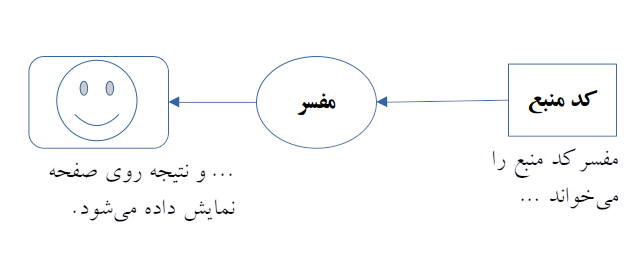
\includegraphics{interpret_fa.eps}
\vspace{0.1in}

A compiler is a program that reads a high-level program and
translates it all at once, before executing any of the commands.
Often you compile the program as a separate step, and then
execute the compiled code later.  In this case, the high-level
program is called the {\bf source code}, and the translated
program is called the {\bf object code} or the {\bf executable}.

As an example, suppose you write a program in C++.  You might
use a text editor to write the program (a text editor is
a simple word processor).  When the program is finished, you
might save it in a file named {\tt program.cpp}, where ``program''
is an arbitrary name you make up, and the suffix {\tt .cpp} is
a convention that indicates that the file contains C++ source
code.

Then, depending on what your programming environment is like,
you might leave the text editor and run the compiler.  The
compiler would read your source code, translate it, and create
a new file named {\tt program.o} to contain the object code,
or {\tt program.exe} to contain the executable. 

\vspace{0.1in}
\centering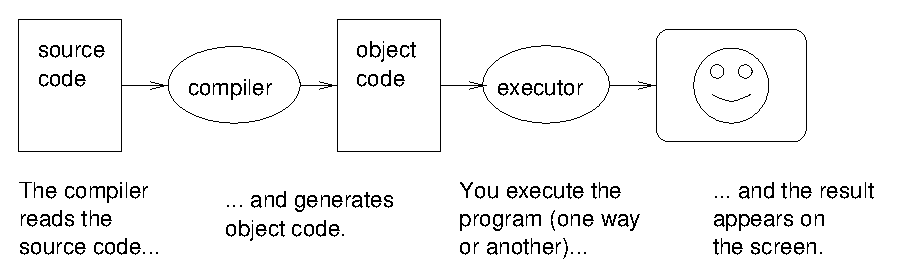
\includegraphics{compile.eps}
\vspace{0.1in}

The next step is to run the program, which requires some kind
of executor.  The role of the executor is to load the program
(copy it from disk into memory) and make the computer start
executing the program.

Although this process may seem complicated, the good news is that in
most programming environments (sometimes called development
environments), these steps are automated for you.  Usually you will
only have to write a program and type a single command to compile and
run it.  On the other hand, it is useful to know what the steps are
that are happening in the background, so that if something goes wrong
you can figure out what it is.

\section{What is a program?}

A program is a sequence of instructions that specifies how to perform
a computation.  The computation might be something mathematical, like
solving a system of equations or finding the roots of a polynomial,
but it can also be a symbolic computation, like searching and
replacing text in a document or (strangely enough) compiling a
program.

\index{statement}

The instructions (or commands, or statements) look different in
different programming languages, but there are a few basic functions
that appear in just about every language:

\begin{description}

\item[input:] Get data from the keyboard, or a file, or some
other device.

\item[output:] Display data on the screen or send data to a
file or other device.

\item[math:] Perform basic mathematical operations like addition and
multiplication.

\item[testing:] Check for certain conditions and execute the
appropriate sequence of statements.

\item[repetition:] Perform some action repeatedly, usually with
some variation.

\end{description}

Believe it or not, that's pretty much all there is to it.
Every program you've ever used, no matter how complicated, is
made up of functions that look more or less like these.  Thus,
one way to describe programming is the process of breaking a
large, complex task up into smaller and smaller subtasks
until eventually the subtasks are simple enough to be performed
with one of these simple functions.

\section{What is debugging?}
\index{debugging}
\index{bug}

Programming is a complex process, and since it is done by
human beings, it often leads to errors.  For whimsical reasons,
programming errors are called {\bf bugs} and the process
of tracking them down and correcting them is called
{\bf debugging}.

There are a few different kinds of errors that can occur
in a program, and it is useful to distinguish between them
in order to track them down more quickly.

\subsection{Compile-time errors}
\index{compile-time error}
\index{error!compile-time}

The compiler can only translate a program if the program is
syntactically correct; otherwise, the compilation fails and
you will not be able to run your program.  {\bf Syntax}
refers to the structure of your program and the rules about
that structure.

\index{syntax}

For example, in English, a sentence must begin with a capital
letter and end with a period.  this sentence contains a syntax
error.  So does this one

For most readers, a few syntax errors are not a significant
problem, which is why we can read the poetry of e e cummings
without spewing error messages.

Compilers are not so forgiving.  If there is a single syntax
error anywhere in your program, the compiler will print an
error message and quit, and you will not be able to run
your program.

To make matters worse, there are more syntax rules in C++
than there are in English, and the error messages you get from
the compiler are often not very helpful.  During the first
few weeks of your programming career, you will probably
spend a lot of time tracking down syntax errors.  As you
gain experience, though, you will make fewer errors and find
them faster.

\subsection{Run-time errors}
\label{run-time}
\index{run-time error}
\index{error!run-time}
\index{safe language}
\index{language!safe}

The second type of error is a run-time error, so-called because
the error does not appear until you run the program.

For the simple sorts of programs we will be writing for the
next few weeks, run-time errors are rare, so it might be a little
while before you encounter one.


\subsection{Logic errors and semantics}
\index{semantics}
\index{logic error}
\index{error!logic}

The third type of error is the {\bf logical} or {\bf semantic}
error.  If there is a logical error in your program, it will
compile and run successfully, in the sense that the computer
will not generate any error messages, but it will not do the
right thing.  It will do something else.  Specifically, it will
do what you told it to do.

The problem is that the program you wrote is not the program
you wanted to write.  The meaning of the program (its semantics)
is wrong.  Identifying logical errors can be tricky, since
it requires you to work backwards by looking at the output
of the program and trying to figure out what it is doing.

\subsection{Experimental debugging}

One of the most important skills you should acquire from working with
this book is debugging.  Although it can be frustrating, debugging is
one of the most intellectually rich, challenging, and interesting
parts of programming.

In some ways debugging is like detective work.  You are
confronted with clues and you have to infer the processes
and events that lead to the results you see.

Debugging is also like an experimental science.  Once you have an idea
what is going wrong, you modify your program and try again.  If your
hypothesis was correct, then you can predict the result of the
modification, and you take a step closer to a working program.  If
your hypothesis was wrong, you have to come up with a new one.  As
Sherlock Holmes pointed out, ``When you have eliminated the
impossible, whatever remains, however improbable, must be the truth.''
(from A. Conan Doyle's {\em The Sign of Four}).

\index{Holmes, Sherlock}
\index{Doyle, Arthur Conan}

For some people, programming and debugging are the
same thing.  That is, programming is the process of gradually
debugging a program until it does what you want.  The idea
is that you should always start with a working program that
does {\em something}, and make small modifications, debugging
them as you go, so that you always have a working program.

For example, Linux is an operating system that contains thousands of
lines of code, but it started out as a simple program Linus Torvalds
used to explore the Intel 80386 chip.  According to Larry Greenfield,
``One of Linus's earlier projects was a program that would switch
between printing AAAA and BBBB.  This later evolved to Linux''
(from {\em The Linux Users' Guide} Beta Version 1).

\index{Linux}

In later chapters I will make more suggestions about debugging
and other programming practices.

\section{Formal and natural languages}
\label{formal}
\index{formal language}
\index{natural language}
\index{language!formal}
\index{language!natural}

{\bf Natural languages} are the languages that people speak,
like English, Spanish, and French.  They were not designed
by people (although people try to impose some order on them);
they evolved naturally.

{\bf Formal languages} are languages that are designed by people for
specific applications.  For example, the notation that mathematicians
use is a formal language that is particularly good at denoting
relationships among numbers and symbols.  Chemists use a formal
language to represent the chemical structure of molecules.  And
most importantly:

\begin{quote}
{\bf Programming languages are formal languages that have been
designed to express computations.}
\end{quote}

As I mentioned before, formal languages tend to have strict rules
about syntax.  For example, $3+3=6$ is a syntactically correct
mathematical statement, but $3=+6\$$ is not.  Also, $H_2O$ is a
syntactically correct chemical name, but $_2Zz$ is not.

Syntax rules come in two flavors, pertaining to tokens and structure.
Tokens are the basic elements of the language, like words and numbers
and chemical elements.  One of the problems with {\tt 3=+6\$} is that
{\tt \$} is not a legal token in mathematics (at least as far as I
know).  Similarly, $_2Zz$ is not legal because there is no element with
the abbreviation $Zz$.

The second type of syntax error pertains to the structure of a
statement; that is, the way the tokens are arranged.  The statement
{\tt 3=+6\$} is structurally illegal, because you can't have a plus
sign immediately after an equals sign.  Similarly, molecular formulas
have to have subscripts after the element name, not before.

When you read a sentence in English or a statement in a formal
language, you have to figure out what the structure of the sentence is
(although in a natural language you do this unconsciously).  This
process is called {\bf parsing}.

\index{parse}

For example, when you hear the sentence, ``The other shoe fell,'' you
understand that ``the other shoe'' is the subject and ``fell'' is the
verb.  Once you have parsed a sentence, you can figure out what it
means, that is, the semantics of the sentence.  Assuming that you know
what a shoe is, and what it means to fall, you will understand the
general implication of this sentence.

Although formal and natural languages have many features in
common---tokens, structure, syntax and semantics---there are many
differences.

\index{ambiguity}
\index{redundancy}
\index{literalness}

\begin{description}

\item[ambiguity:] Natural languages are full of ambiguity, which
people deal with by using contextual clues and other information.
Formal languages are designed to be nearly or completely unambiguous,
which means that any statement has exactly one meaning,
regardless of context.

\item[redundancy:] In order to make up for ambiguity and reduce
misunderstandings, natural languages employ lots of
redundancy.  As a result, they are often verbose.  Formal languages
are less redundant and more concise.

\item[literalness:] Natural languages are full of idiom and
metaphor.  If I say, ``The other shoe fell,'' there is probably
no shoe and nothing falling.  Formal languages mean
exactly what they say.

\end{description}

People who grow up speaking a natural language (everyone) often have a
hard time adjusting to formal languages.  In some ways the difference
between formal and natural language is like the difference between
poetry and prose, but more so:

\index{poetry}
\index{prose}

\begin{description}

\item[Poetry:] Words are used for their sounds as well as for
their meaning, and the whole poem together creates an effect or
emotional response.  Ambiguity is not only common but often
deliberate.

\item[Prose:] The literal meaning of words is more important
and the structure contributes more meaning.  Prose is more amenable to
analysis than poetry, but still often ambiguous.

\item[Programs:] The meaning of a computer program is unambiguous
and literal, and can be understood entirely by analysis of the
tokens and structure.

\end{description}

Here are some suggestions for reading programs (and other formal
languages).  First, remember that formal languages are much more dense
than natural languages, so it takes longer to read them.  Also, the
structure is very important, so it is usually not a good idea to read
from top to bottom, left to right.  Instead, learn to parse the
program in your head, identifying the tokens and interpreting the
structure.  Finally, remember that the details matter.  Little things
like spelling errors and bad punctuation, which you can get away
with in natural languages, can make a big difference in a formal
language.

\section{The first program}
\label{hello}
\index{hello world}

Traditionally the first program people write in a new language
is called ``Hello, World.'' because all it does is print the
words ``Hello, World.''  In C++, this program looks like this:

\begin{lstlisting}
#include <iostream>
using namespace std;

// main: generate some simple output

int main ()
{
  cout << "Hello, world." << endl;
  return 0;
}
\end{lstlisting}
%
Some people judge the quality of a programming language by
the simplicity of the ``Hello, World.'' program.  By this
standard, C++ does reasonably well.  Even so, this simple
program contains several features that are hard to explain to
beginning programmers.  For now, we will ignore some of
them, like the first two lines.

\index{comment}
\index{statement!comment}

The third line begins with {\tt //}, which indicates
that it is a {\bf comment}.  A comment is a bit of
English text that you can put in the middle of a program,
usually to explain what the program does.  When the compiler
sees a {\tt //}, it ignores everything from there until the end
of the line.

In the fourth line, you can ignore the word {\tt int}
for now, but notice the word {\tt main}.  {\tt main} is a
special name that indicates the place in the program where execution
begins.  When the program runs, it starts by executing the first
statement in {\tt main} and it continues, in order, until it gets
to the last statement, and then it quits.

\index{output}
\index{statement!output}

There is no limit to the number of statements that can be in {\tt
main}, but the example contains only one.  It is a basic {\bf
output} statement, meaning that it outputs or displays a message on
the screen.  

{\tt cout} is a special object provided by the system to allow
you to send output to the screen.  The symbol {\tt <<} is an
{\bf operator} that you apply to {\tt cout} and a string, and that
causes the string to be displayed.

\index{operator}

{\tt endl} is a special symbol that represents the end of a
line.  When you send an {\tt endl} to {\tt cout}, it causes the
cursor to move to the next line of the display.
The next time you output something, the new text appears
on the next line.

Like all statements, the output statement ends with a
semi-colon ({\tt ;}).

There are a few other things you should notice about the syntax of
this program.  First, C++ uses squiggly-braces (\{ and
\}) to group things together.  In this case, the output statement
is enclosed in squiggly-braces, indicating that it is {\em inside} the
definition of {\tt main}.  Also, notice that the statement is
indented, which helps to show visually which lines are inside the
definition.

At this point it would be a good idea to sit down in front of
a computer and compile and run this program.  The details of how
to do that depend on your programming environment, but from now
on in this book I will assume that you know how to do it.

As I mentioned, the C++ compiler is a real stickler for syntax.
If you make any errors when you type in the program, chances
are that it will not compile successfully.  For example, if
you misspell {\tt iostream}, you might get an error message like
the following:

\begin{verbatim}
hello.cpp:1: oistream.h: No such file or directory
\end{verbatim}
%
There is a lot of information on this line, but it is presented
in a dense format that is not easy to interpret.  A more friendly
compiler might say something like:

\begin{quote}
``On line 1 of the source code file named hello.cpp, you tried to
include a header file named oistream.h.  I didn't find anything
with that name, but I did find something named iostream.  Is
that what you meant, by any chance?''
\end{quote}

Unfortunately, few compilers are so accomodating.  The compiler
is not really very smart, and in most cases the error message
you get will be only a hint about what is wrong.  It will take
some time to gain facility at interpreting compiler messages.

Nevertheless, the compiler can be a useful tool for learning the
syntax rules of a language.  Starting with a working program
(like hello.cpp), modify it in various ways and see what happens.
If you get an error message, try to remember what the message says
and what caused it, so if you see it again in the future you
will know what it means.

\section{Glossary}

\begin{description}

\item[problem-solving:]  The process of formulating a problem, finding
a solution, and expressing the solution.

\item[high-level language:]  A programming language like C++ that
is designed to be easy for humans to read and write.

\item[low-level language:]  A programming language that is designed
to be easy for a computer to execute.  Also called ``machine
language'' or ``assembly language.''

\item[portability:]  A property of a program that can run on more
than one kind of computer.

\item[formal language:]  Any of the languages people have designed
for specific purposes, like representing mathematical ideas or
computer programs.  All programming languages are formal languages.

\item[natural language:]  Any of the languages people speak that
have evolved naturally.

\item[interpret:]  To execute a program in a high-level language
by translating it one line at a time.

\item[compile:]  To translate a program in a high-level language
into a low-level language, all at once, in preparation for later
execution.

\item[source code:]  A program in a high-level language, before
being compiled.

\item[object code:]  The output of the compiler, after translating
the program.

\item[executable:]  Another name for object code that is ready
to be executed.

\item[algorithm:]  A general process for solving a category of
problems. 

\item[bug:]  An error in a program.

\item[syntax:]  The structure of a program.

\item[semantics:]  The meaning of a program.

\item[parse:]  To examine a program and analyze the syntactic structure.

\item[syntax error:]  An error in a program that makes it impossible
to parse (and therefore impossible to compile).

\item[run-time error:]  An error in a program that makes it fail at
run-time.

\item[logical error:]  An error in a program that makes it do something
other than what the programmer intended.

\item[debugging:]  The process of finding and removing any of
the three kinds of errors.

\index{problem-solving}
\index{high-level language}
\index{low-level language}
\index{formal language}
\index{natural language}
\index{interpret}
\index{compile}
\index{syntax}
\index{semantics}
\index{parse}
\index{error}
\index{debugging}

\end{description}





\appendix
% LaTeX source for textbook ``How to think like a computer scientist''
% Copyright (C) 1999  Allen B. Downey


\chapter{Quick reference for AP classes}

These class definitions are copied from the College Board
web page,

\begin{verbatim}
http://www.collegeboard.org/ap/computer-science/html/quick_ref.htm
\end{verbatim}

with minor formatting changes.  This is probably a good time to
repeat the following text, also from the College Board web page.

\begin{quotation}
"Inclusion of the C++ classes defined for use in the Advanced
Placement Computer Science courses does not constitute endorsement of
the other material in this textbook by the College Board, Educational
Testing service, or the AP Computer Science Development Committee. The
versions of the C++ classes defined for use in the AP Computer Science
courses included in this textbook were accurate as of 20 July
1999.  Revisions to the classes may have been made since that time."
\end{quotation}

\section{{\tt apstring}}

\begin{verbatim}
extern const int npos;  // used to indicate not a position in the string

// public member functions

  // constructors/destructor
  apstring();                       // construct empty string ""
  apstring(const char * s);         // construct from string literal
  apstring(const apstring & str);   // copy constructor
  ~apstring();                      // destructor

  // assignment
  const apstring & operator= (const apstring & str); // assign str
  const apstring & operator= (const char * s);       // assign s
  const apstring & operator= (char ch);              // assign ch

  // accessors
  int length() const;                      // number of chars
  int find(const apstring & str) const;    // index of first occurrence of str
  int find(char ch) const;                 // index of first occurrence of ch
  apstring substr(int pos, int len) const; // substring of len chars, 
                                           // starting at pos
  const char * c_str() const;              // explicit conversion to char *

  // indexing
  char operator[ ](int k) const; // range-checked indexing
  char & operator[ ](int k);     // range-checked indexing

  // modifiers
  const apstring & operator+= (const apstring & str); // append str
  const apstring & operator+= (char ch);              // append char

  // The following free (non-member) functions operate on strings

  // I/O functions
  ostream & operator<< ( ostream & os, const apstring & str );
  istream & operator>> ( istream & is, apstring & str );
  istream & getline( istream & is, apstring & str );

  // comparison operators
  bool operator== ( const apstring & lhs, const apstring & rhs );
  bool operator!= ( const apstring & lhs, const apstring & rhs );
  bool operator<  ( const apstring & lhs, const apstring & rhs );
  bool operator<= ( const apstring & lhs, const apstring & rhs );
  bool operator>  ( const apstring & lhs, const apstring & rhs );
  bool operator>= ( const apstring & lhs, const apstring & rhs );

  // concatenation operator +
  apstring operator+ ( const apstring & lhs, const apstring & rhs );
  apstring operator+ ( char ch, const apstring & str );
  apstring operator+ ( const apstring & str, char ch );
\end{verbatim}

\section{{\tt apvector}}

\begin{verbatim}
template <class itemType>
class apvector

// public member functions

  // constructors/destructor
  apvector();                                 // default constructor (size==0)
  apvector(int size);                         // initial size of vector is size
  apvector(int size, const itemType & fillValue);  // all entries == fillValue
  apvector(const apvector & vec);             // copy constructor
  ~apvector();                                // destructor

  // assignment
  const apvector & operator= (const apvector & vec);

  // accessors
  int length() const;                            // capacity of vector

  // indexing
  // indexing with range checking
  itemType & operator[ ](int index);           
  const itemType & operator[ ](int index) const;

  // modifiers
  void resize(int newSize);               // change size dynamically
                                          //can result in losing values
\end{verbatim}

\section{{\tt apmatrix}}

\begin{verbatim}
template <class itemType>
class apmatrix

// public member functions

  // constructors/destructor
  apmatrix();                                   // default size is 0 x 0
  apmatrix(int rows, int cols);                 // size is rows x cols
  apmatrix(int rows, int cols, const itemType & fillValue);
                                                // all entries == fillValue
  apmatrix(const apmatrix & mat);               // copy constructor
  ~apmatrix( );                                 // destructor

  // assignment
  const apmatrix & operator = (const apmatrix & rhs);

  // accessors
  int numrows() const;                                  // number of rows
  int numcols() const;                                  // number of columns

  // indexing
  // range-checked indexing
  const apvector<itemType> & operator[ ](int k) const;  
  apvector<itemType> & operator[ ](int k);

  // modifiers
  void resize(int newRows, int newCols); // resizes matrix to newRows x newCols
                                         // (can result in losing values)
\end{verbatim}



\printindex

\end{document}


